\chapter{Segmentation}
The goal of segmentation is to partition data into meaningful subsets. In heritage range images such groupings often include, but are not limited to: points representing vegetation, walls, people or scanner artifacts. Isolating these points can be extremely difficult and time consuming. Suitable segmentation techniques for heritage cleaning should speed up the process by reducing a user's workload while maintaining interactivity.

% Interactive batch jobs

\section{Performance}
A key metric for measuring the utility of a technique is the time it takes to achieve a segmentation result. The total segmentation time is the sum of durations associated with each action. The time to perform a segmentation can thus be reduced by either minimizing the time consumed by individual actions or reducing the number of actions.

Reduction in the time consumed by an for user actions can be achieved via a good user interface, as discussed in \ref{chapter:framework}.The number of actions required by a user can be reduced by delegating work to an algorithm. It is important for an effective algorithm to produce a result within a reasonable amount of time. If a user could achieve an equivalent result without the algorithm in less time, the technique adds no value.

For non-synthetic range images, it is unlikely that an algorithm will produce a perfect segmentation. It is thus expected that remedial action by a user will almost always be required. The final segmentation will thus be the total time required by each algorithm action and remedial user actions.

\begin{figure}[ht]
  \centering
  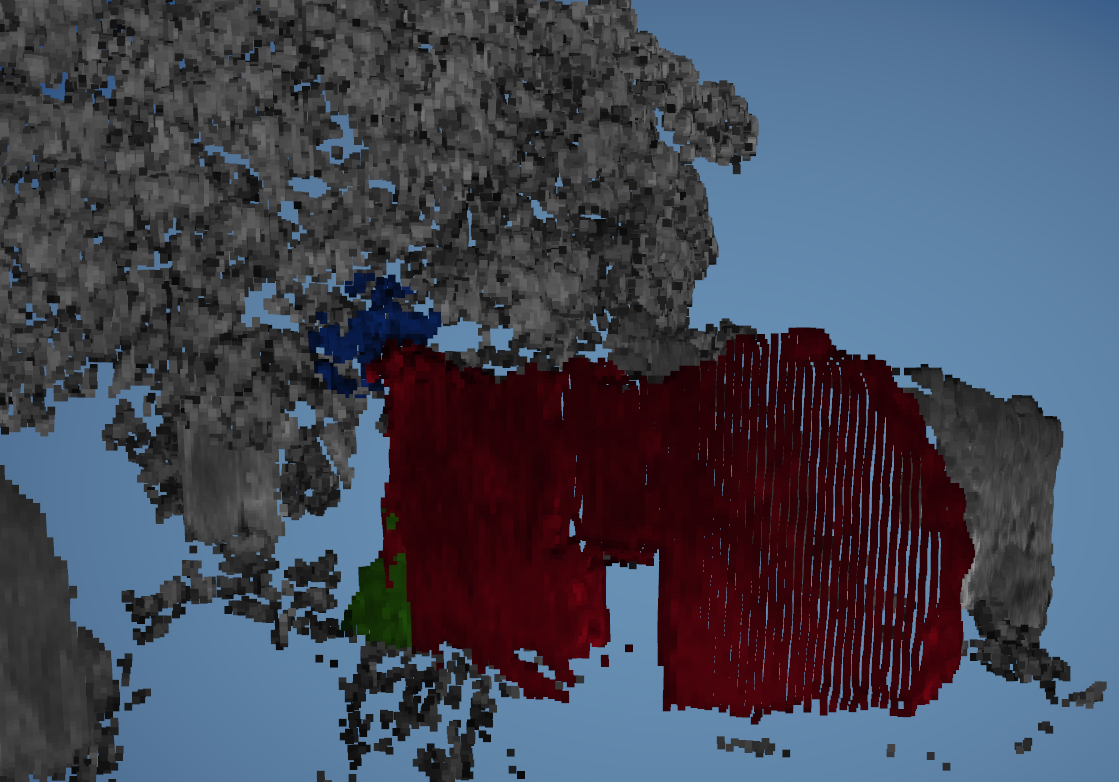
\includegraphics[width=1\linewidth]{images/walltree.png}
  \caption[Imperfect segmentation]{Example of a imperfect segmentation. The wall (red and green region) was targeted but the red and blue region were selected. In order the produce the correct wall segmentation, a user will need to deselect the blue region (false positive), and select the green region (false negative) } 
  \label{fig:imperfectseg}
\end{figure}

For example, if an automated tool for wall segmentation selected 95\% of the wall and part of a nearby tree, a complete segmentation will only be achieved once the remaining 5\% of the wall is selected and the tree points removed (see \autoref{fig:imperfectseg}). If a user could previously perform the segmentation in 2 minutes, the automated tool would only be effective if it could allow a user complete the task in less than 2 minutes. If the wall segmentation tool needs 30 seconds to isolate the wall and then requires and additional 30 seconds of user action to refine the result, the tool can be considered useful as it can reduce the segmentation time by 1 minute. If however, the accuracy of the result is such that an additional 2 minutes of user action is required to achieve the same result, the tool provides no advantage over the status quo. The same can be said if the processing time pushed the total time over the 2 minute mark.

A high accuracy technique can minimize the amount of subsequent remedial user action required following its use. It should, however, be noted that accuracy is not directly related to reduced effort. Consider a wall selection tool that selects 50\% of a target wall. If the tool selected hard to isolate points and the remaining points could easily be selected with a single user action, the total time could still be low. This wall selection tool would exhibit low accuracy but would still be effective.


\section{Evaluation}

\begin{figure}[ht]
  \centering
  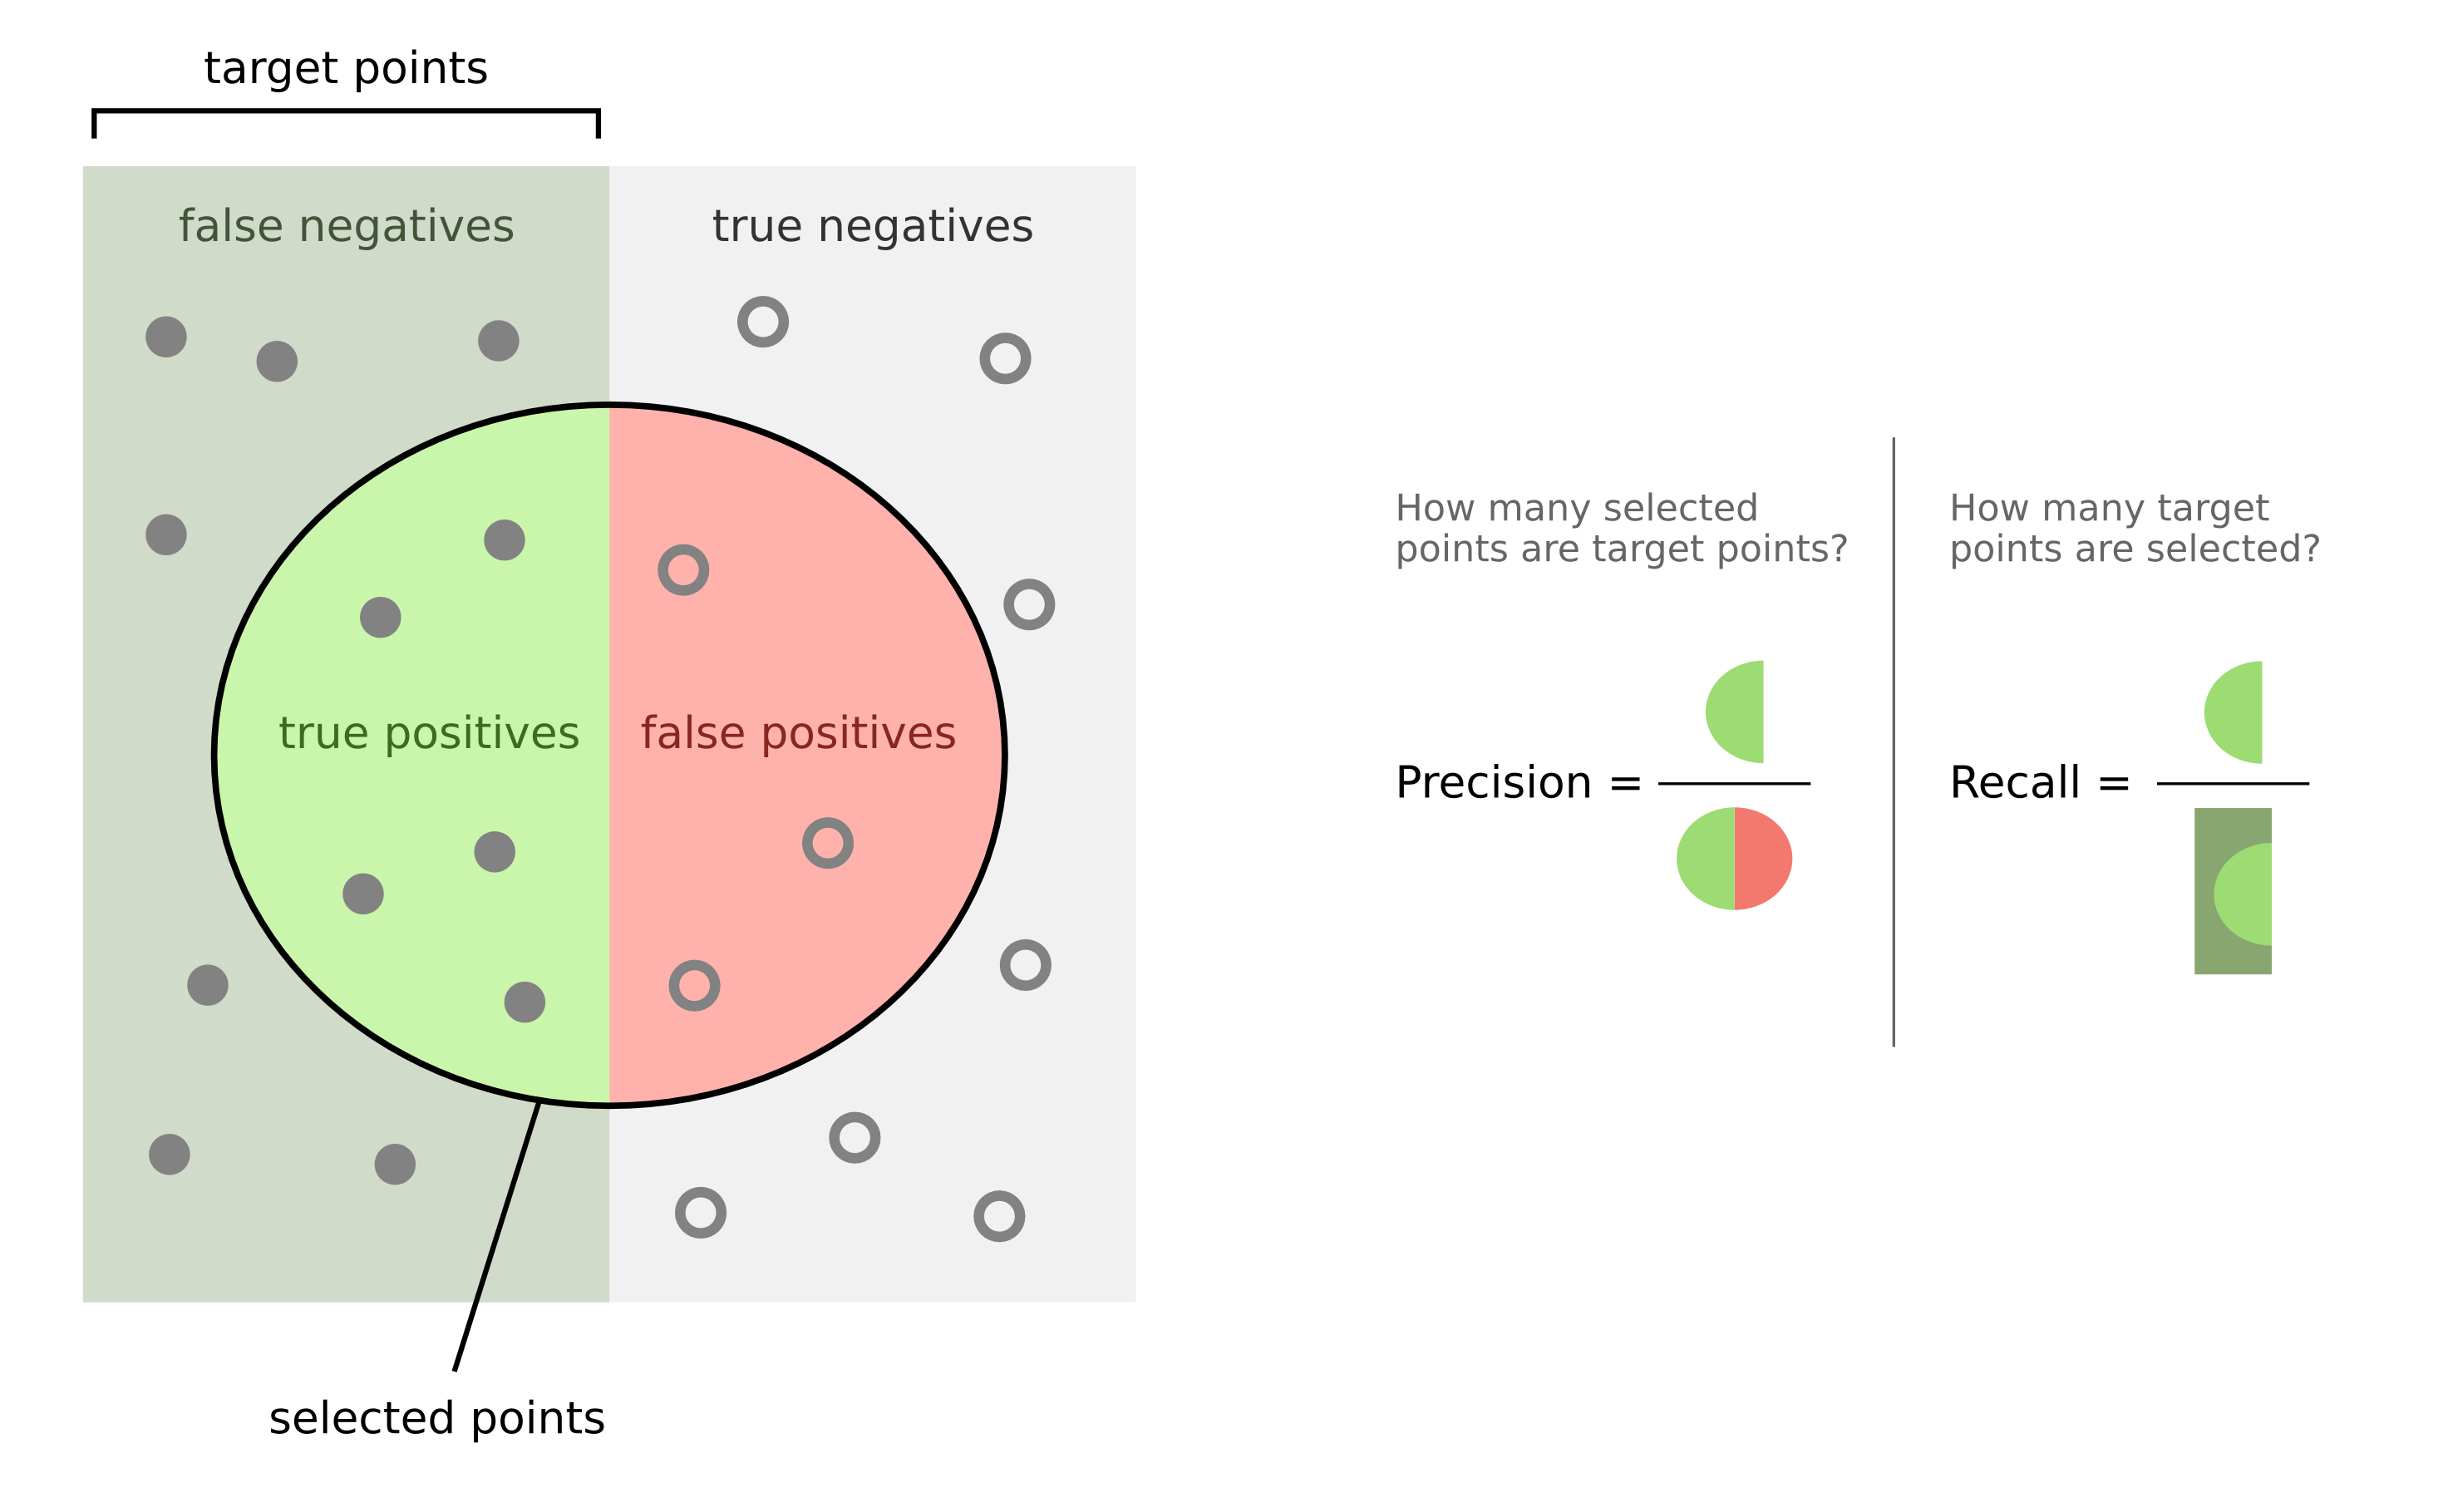
\includegraphics[width=1\linewidth]{images/precision_recall.png}
  \caption[Precision and recall]{Precision and recall \protect\footnotemark } 
  \label{fig:precision_recall}
\end{figure}
\footnotetext{Adapted from: \url{https://en.wikipedia.org/wiki/Precision\_and\_recall}}

Segmentation algorithms are typically evaluated in terms of precision and recall \cite{Ponce2012}. Given a set of points we define a subset as our target. If an algorithm selects another subset, the selected points can be divided into true positives and false negatives. The remaining points are either false negatives or true negatives (see \autoref{fig:precision_recall}).

Precision is then defined as the number of true positives selected as fraction of the total number of selected points.

\begin{equation} \label{eq:precision}
	\text{precision}=\frac{|\{\text{target points}\}\cap\{\text{selected points}\}|}{|\{\text{selected points}\}|}
   % \right.
\end{equation}

Recall is defined as the number of true positives as a fraction of the targeted points.

\begin{equation} \label{eq:recall}
	\text{recall}=\frac{|\{\text{target points}\}\cap\{\text{selected points}\}|}{|\{\text{selected points}\}|}
   % \right.
\end{equation}

These two measures can be combined as an F-score that represents accuracy. The score can be interpreted as the weighted average of precision and recall.

\begin{equation} \label{eq:f1score}
	F_1 = 2 \cdot \frac{\mathrm{precision} \cdot \mathrm{recall}}{\mathrm{precision} + \mathrm{recall}}
   % \right.
\end{equation}

Our position is unique in that user efficiency instead of accuracy is our primary objective. Accuracy is still a good indicator of how useful related research is likely to be. Computational efficiency however is at least as important as it contributes to the total task time.

\section{Evaluation technique}
In order to evaluate how effective a segmentation method is we need to know how long it will take a user to produce a segmentation given the method and how long a user will take without it. User testing is however time consuming and expensive. Instead of user testing we choose to develop a technique to simulates a user's segmentation actions.

The technique requires reference segmentation which is used to compute a series of user actions to reproduce the result. The reference segmentation can be reproduced from the ground up or from a pre-existing segmentation. Associating a time value with each user action allows us to estimate the time required to reproduce a reference segmentation.

In a real world cleaning task, users may have access to a variety of tools that work best in certain situations. Determining when a simulated user should use one tool over another may be difficult. Settling on a single tool allows us to drastically reduce simulation complexity. We have found, at one organisation, that point cloud cleaning was performed with the use of only a polygon select tool. While this may not be ideal, it does boost the ecological validity of a simplified single tool simulation. For this reason our simulation uses a polygon select tool.

As previously discussed, a polygon lasso tool is not ideal in situations where a target cannot easily be isolated. In 3D, a user can view the target from a position that minimizes the number of false selections (see \autoref{fig:3dselect}). Finding such an ideal vantage point would add significant computational complexity to a simulation. Instead, our simulation computes polygon selections in 2D. This allows us to avoid false selections of points behind the target. It can however result in more false selections of surrounding points (see \autoref{fig:2dselect}).

\begin{figure}
\centering
\begin{subfigure}{.33\textwidth}
  \centering
  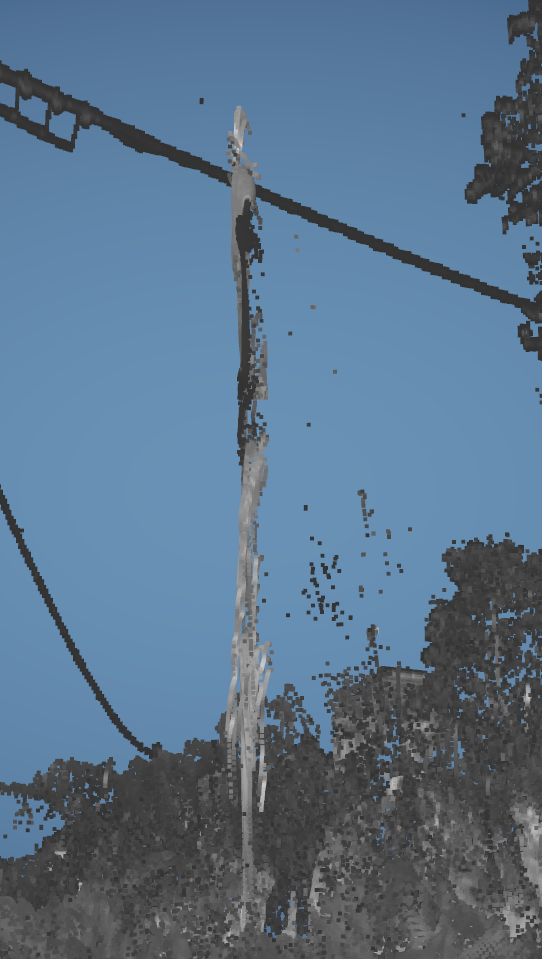
\includegraphics[height=6cm]{images/3dselect/1.png}
  \captionsetup{margin=5pt}
  \caption{This perspective makes it hard to avoid cable selection}
\end{subfigure}%
\begin{subfigure}{.33\textwidth}
  \centering
  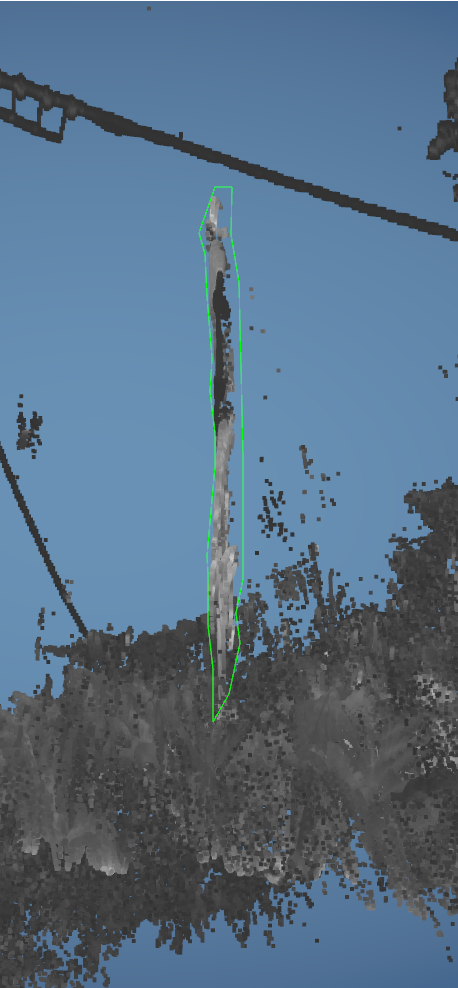
\includegraphics[height=6cm]{images/3dselect/2.png}
  \captionsetup{margin=5pt}
  \caption{False selection can be avoided via a different perspective}
\end{subfigure}
\begin{subfigure}{.33\textwidth}
  \centering
  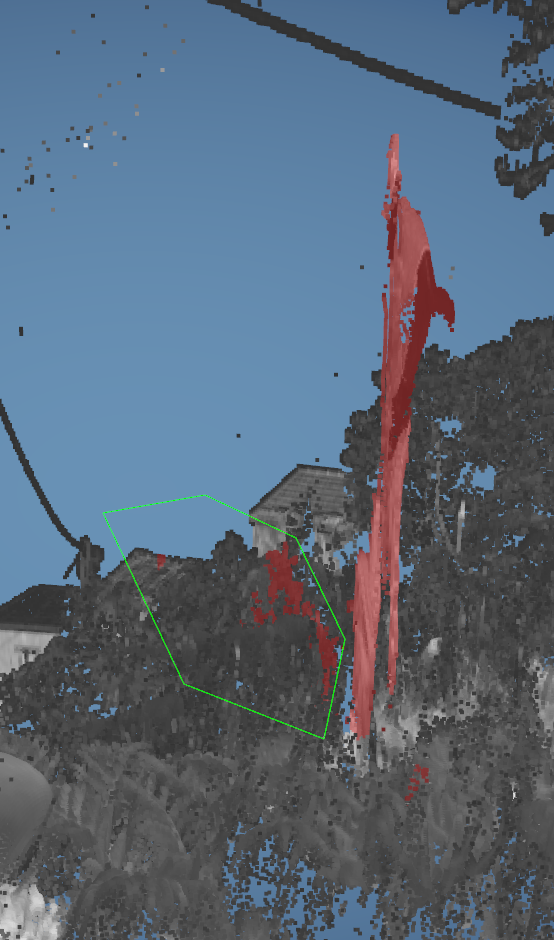
\includegraphics[height=6cm]{images/3dselect/3.png}
  \captionsetup{margin=5pt}
  \caption{False selection were not completely avoided and requires remedial action}
\end{subfigure}
\caption{3D polygon selection}\label{fig:3dselect}
\end{figure}


\begin{figure}
\centering
\begin{subfigure}{.3\textwidth}
  \centering
  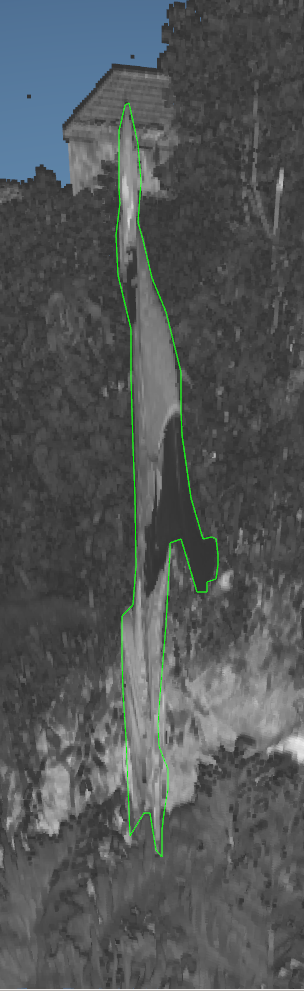
\includegraphics[height=6cm]{images/2dselect/1.png}
  \caption{Polygon around target}
\end{subfigure}%
\begin{subfigure}{.3\textwidth}
  \centering
  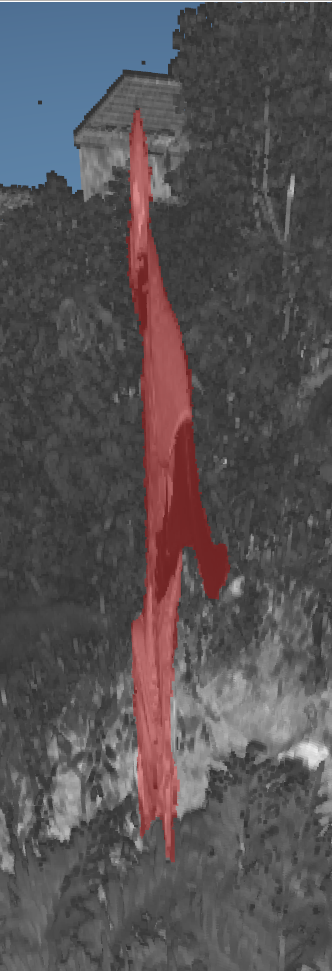
\includegraphics[height=6cm]{images/2dselect/2.png}
  \caption{Resultant selection}
\end{subfigure}
\begin{subfigure}{.3\textwidth}
  \centering
  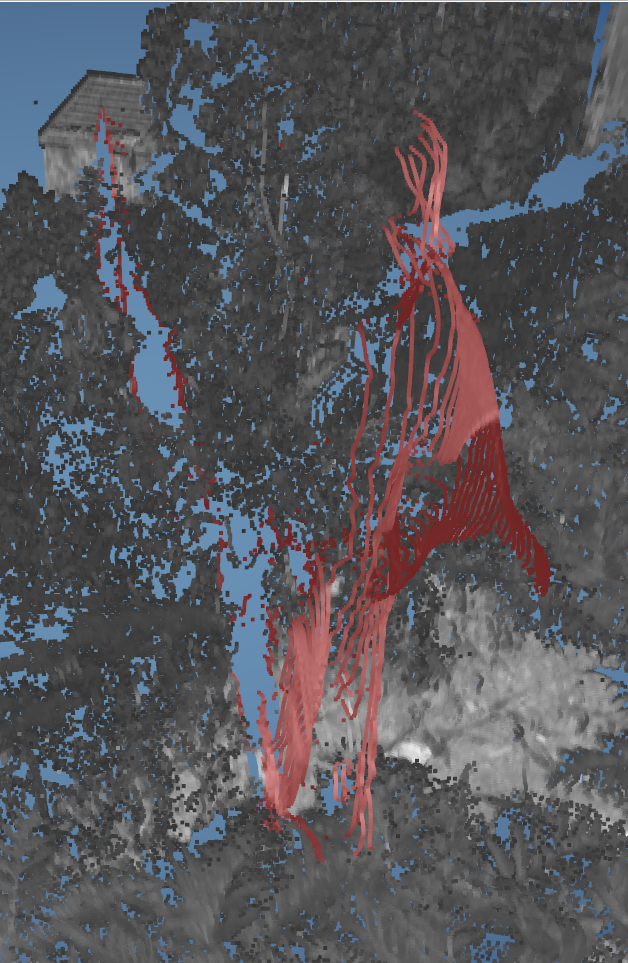
\includegraphics[height=6cm]{images/2dselect/3.png}
  \caption{False positives are identifiable from a different perspective}
\end{subfigure}
\caption{2D polygon selection}\label{fig:2dselect}
\end{figure}


The first step in emulating the polygon selection tool is to find groups of points, within the reference set, that the user is likely to target (see \autoref{fig:clusters}). A simple 2D euclidean clustering algorithm achieves this \cite{Rusu2009a}. The clustering algorithm uses KD-tree to grow a region as long as the next point is within a threshold distance of the last. The minimum size of a cluster also needs to be specified.

Given a cluster, the boundary is established by computing a concave hull \cite{Moreira2006} (see \autoref{fig:concavehull}). The algorithm used is a variation of the gift-wrapping convex hull algorithm \cite{Jarvis1973}. First, an extrema in the y or x axis is found. The K-nearest neighbours at the extrema are then computed. The first edge of the hull is created between the extrema and the neighbour that makes the biggest right hand turn relative to the extrema axis. The next point is selected in the same manner but the right hand turn is measured relative to the previous edge. Each edge, other than the starting edge, can only be visited once. When the starting point is reached again the hull is complete. The starting vertex can only be revisited after the 3rd iteration. This ensures that the algorithm does not terminate prematurely. The K that is chosen for the neighbour search affects how dense the hull is and how many outliers are excluded.

The computed hull around a cluster usually consist of a large number of boundary points. A human is unlikely to use as many points or be as precise. The number of points are reduced by applying a polygon simplification algorithm \cite{Ramer1972} (see \autoref{fig:simplification}). The simplification algorithm ensures that for any point P in between points A and B on the polygon, the distance to line AB from C will be greater than a given threshold. If this is not true the point is removed.

The simplification algorithm may shrink the hull and produce false negatives. The hull can, however, only shrink in proportion to the threshold selected for the simplification. To compensate for the reduced size the hull can be expanded proportionally outwards (see \autoref{fig:expand}). Each point in the hull is moved outwards along the 2D point normal. The adjustment needs to be such that the false positive are minimised.


\begin{figure}
\centering
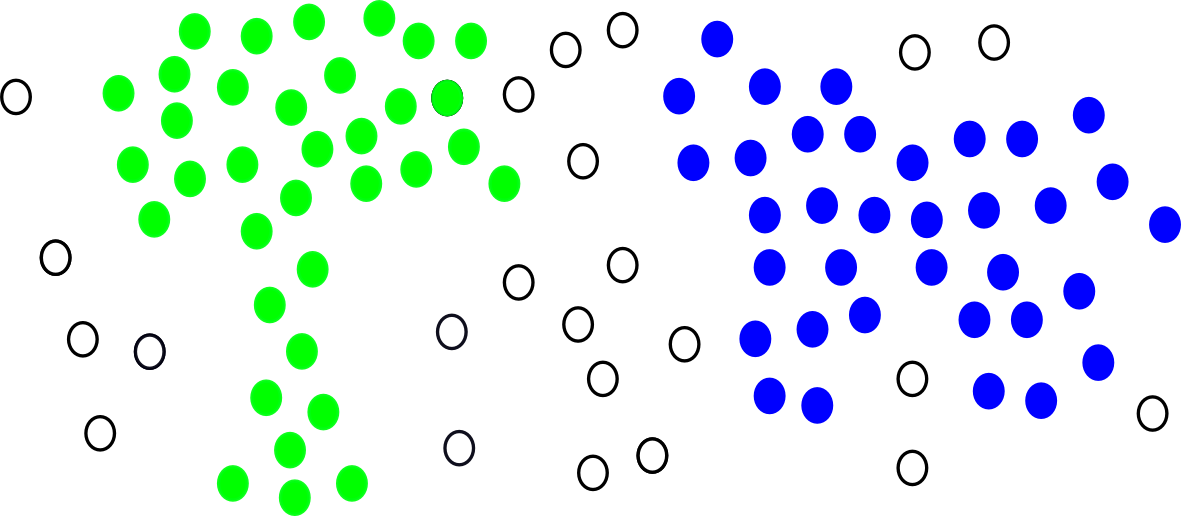
\includegraphics[height=4cm]{images/evaltool/scan.png}
\caption[Clustering step]{Clustering the reference segmentation (black dots) into 2 clusters (green and blue dots)}\label{fig:clusters}
\end{figure}


\begin{figure}
\centering
\begin{subfigure}{.3\textwidth}
  \centering
  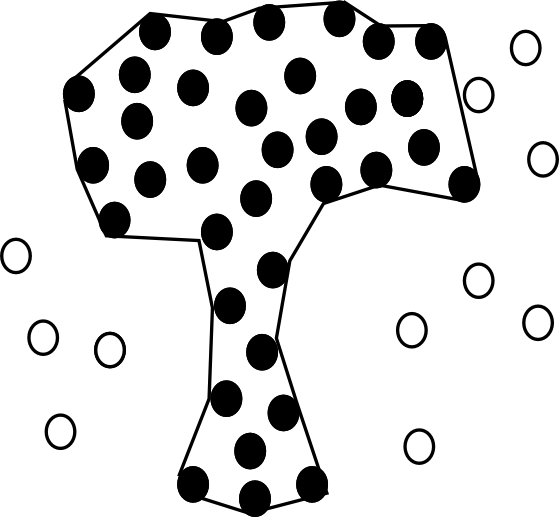
\includegraphics[height=3cm]{images/evaltool/tree1.png}
  \captionsetup{margin=5pt}
  \caption{Concave hull}
  \label{fig:concavehull}
\end{subfigure}%
\begin{subfigure}{.3\textwidth}
  \centering
  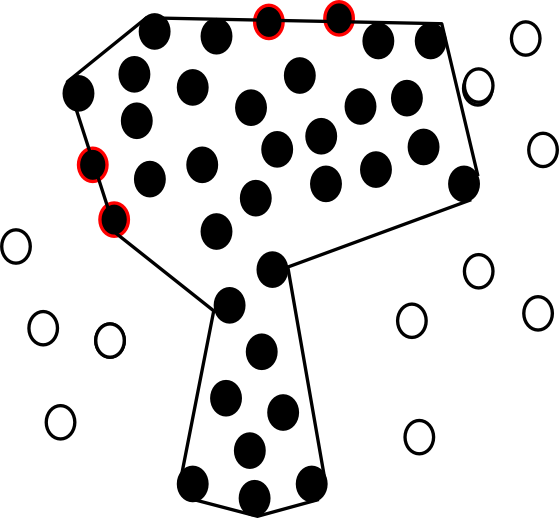
\includegraphics[height=3cm]{images/evaltool/tree2.png}
  \captionsetup{margin=5pt}
  \caption{Polygon simplification. This step can create false negatives (black and red dots)}
  \label{fig:simplification}
\end{subfigure}
\begin{subfigure}{.3\textwidth}
  \centering
  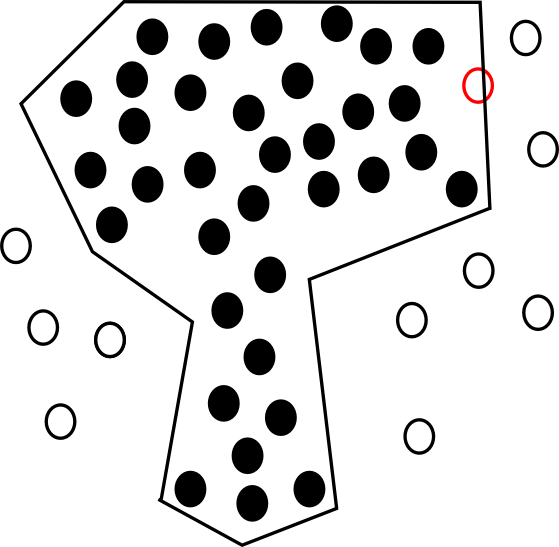
\includegraphics[height=3cm]{images/evaltool/tree3.png}
  \captionsetup{margin=5pt}
  \caption{Dilating the simplified hull. False negatives (red and white dots) can be added by this step}
  \label{fig:expand}
\end{subfigure}
\caption{Creating a realistic polygon around the first cluster}
\label{fig:polygoncluster}
\end{figure}



\begin{figure}
\centering
\begin{subfigure}{.3\textwidth}
  \centering
  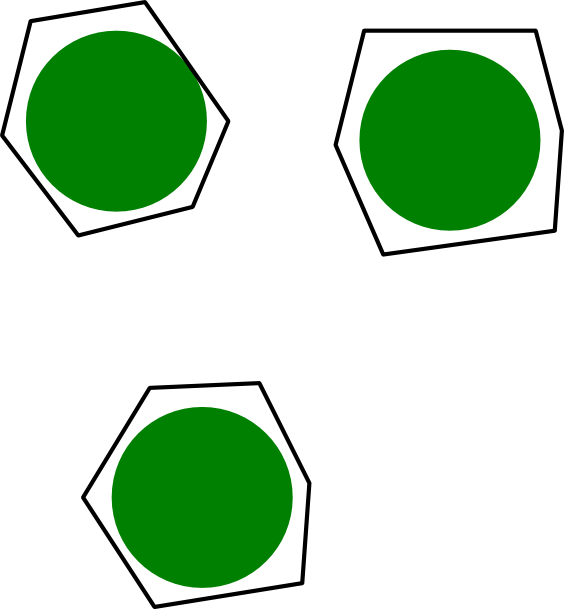
\includegraphics[height=4cm]{images/evaltool/individual.png}
  \caption{Individual cluster selection}
  \label{fig:individualclusters}
\end{subfigure}%
\begin{subfigure}{.3\textwidth}
  \centering
  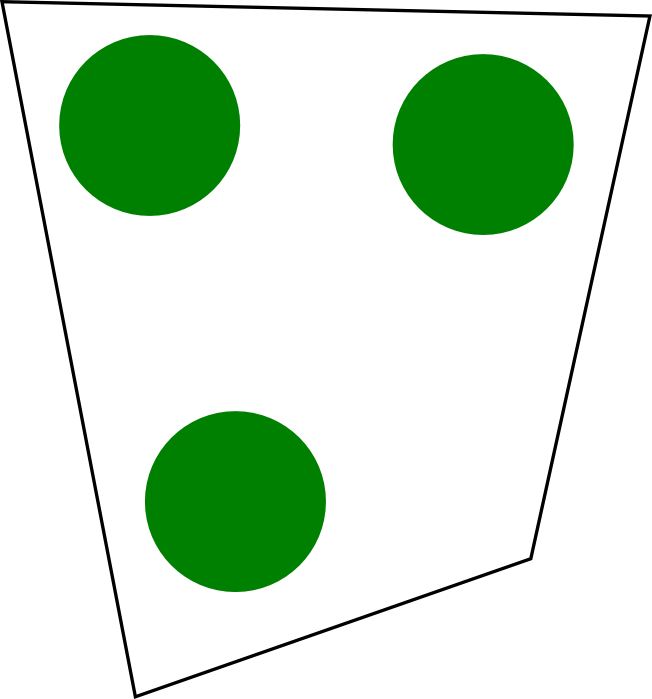
\includegraphics[height=4cm]{images/evaltool/goodselect.png}
  \caption{Multi cluster selection}
  \label{fig:multicluster}
\end{subfigure}%
\begin{subfigure}{.3\textwidth}
  \centering
  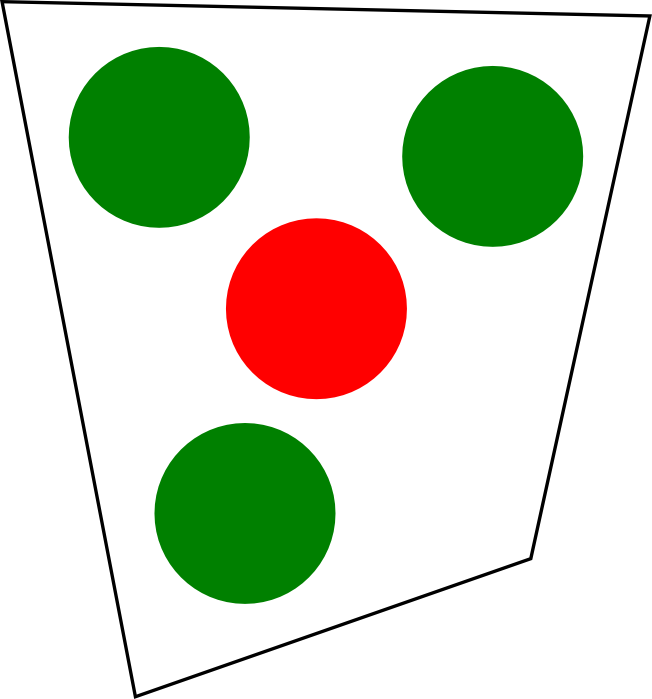
\includegraphics[height=4cm]{images/evaltool/badselect.png}
  \caption{Multi cluster selection results in a false positive}
  \label{fig:badmulticluster}
\end{subfigure}
\caption{Selecting multiple clusters}\label{multiselect}
\label{fig:test}
\end{figure}



The previous steps assume the user will select each cluster individually (see \autoref{fig:individualclusters}). This assumption does not always hold true. In a real world task, less effort may be required to select multiple clusters of points with a single polygon (see \autoref{fig:multicluster}). However, if the polygon around the clusters result in a false positive or negative selection (see \autoref{fig:badmulticluster}), further actions will be required to correct it. It therefore needs be determined whether the larger selection followed by remedial actions, or individual selections, are less less effortful.

After computing polygons for each cluster, we determine if multiple clusters can be selected with a single polygon. To do this each pair of polygons are merged by computing their combined convex hull \cite{Andrew1979}. We then check if the selection produced by the combined hull creates false selections in addition to those produced by the individual hulls. If the false selections are below a threshold the two hulls are replaced by the merged hull. These steps are repeated on all subsequent hull pairs. 

The steps described above will produce false selections. To improve accuracy, false positive and false negative points are clustered and the algorithm is repeated. Hulls associated with false negative points will be selected and those associated with false positive points will be deselected. This process can be repeated until a predetermined level of accuracy is reached. This is analogous to the refinement that takes place into real point cloud cleaning.

While each iteration may improve the accuracy of the segmentation, the extra simulated effort may not be worth the marginal increase in accuracy. An iteration can also produce as many false positives as the false negatives that were eliminated. The algorithm should thus terminate either when a set accuracy is reached, or the marginal improvement is not sufficient to justify the additional effort.

\begin{algorithm}
  \caption{Lasso tool simulation\label{alg:eval}}
  \begin{algorithmic}[1]
    \Let{$simplificationFactor$}{$5$}
    \Let{$falseSelectionCount$}{\Call{countFalseSelection}{$selection, target$}}
    \Let{$iterations$}{$0$}
    \While{$falseSelectionCount > threshold$ $\|$ $iterations <maxItterations$}
      \Let{$falsePositives$}{$selection - target$}
      \Let{$falseNegatives$}{$selection \cap target^c$}

      \Let{$fpClusters$}{\Call{Cluster}{$falsePositives$}}
      \Let{$fnClusters$}{\Call{Cluster}{$falsePegatives$}}

      \Let{$fpHulls$}{\Call{ConvexHull}{$fpClusters$}}
      \Let{$fnHulls$}{\Call{ConvexHull}{$fnClusters$}}

      \State\Call{Simplify}{$fpHulls, simplificationFactor$}
      \State\Call{Simplify}{$fnHulls, simplificationFactor$}

      \State\Call{Expand}{$fpHulls, simplificationFactor$}
      \State\Call{Expand}{$fnHulls, simplificationFactor$}

      \For{$ i \gets 0 \textrm{ to } fpHulls.length$} \Comment{Merge hulls}
        \For{$ j \gets i \textrm{ to } fpHulls.length$}
          \Let{$combined$}{\Call{Merge}{$fpHulls_i, fpHulls_j$}}
          \If{\Call{HasFalseSelection}{$combined, target$}}
            \Let{$fpHulls_i$}{$combined$}
            \State $fpHulls.remove(j)$
            \Let{$j$}{$j - 1$}
          \EndIf
        \EndFor
      \EndFor

      \For{$ i \gets 0 \textrm{ to } fnHulls.length$} \Comment{Merge hulls}
        \For{$ j \gets i \textrm{ to } fnHulls.length$}
          \Let{$combined$}{\Call{Merge}{$fnHulls_i, fnHulls_j$}}
          \If{\Call{HasFalseSelection}{$combined, target$}}
            \Let{$fnHulls_i$}{$combined$}
            \State $fnHulls.remove(j)$
            \Let{$j$}{$j - 1$}
          \EndIf
        \EndFor
      \EndFor

      \State\Call{Deselect}{$fphulls$}
      \State\Call{Select}{$fnhulls$}
      \Let{$itterations$}{$itterations + 1$}
      \Let{$falseSelectionCount$}{\Call{countFalseSelection}{$selection, target$}}
    \EndWhile


  \end{algorithmic}
\end{algorithm}

\todo{How is this determined}

\subsection{Metrics and ecological validity}
To estimate the time a user will take to reproduce a segmentation, we need to associate a time value with the placement of each vertex in a polygon. The overhead associated with starting and finalising each polygon also needs to be determined.

To correctly estimate the total segmentation time, the algorithm actions need to mirror user's polygon and vertex counts. We can modify the number of vertices in a polygon by setting the threshold of the polygon approximation algorithm. The number polygons constructed can be adjusted by modifying the termination condition.\todo{clarify}

Test data was collected by asking users to segment five objects of varying complexity in a pilot study of five users \cite{Mathematical1910}. Users were shown the reference segmentation before starting each scan and asked to obtain a similar level of detail. The time users took to invoke and finalise each polygon was recorded, as well as the number of points in each polygon and time to draw each polygon. The recall and precision for each segmentation was also recorded.

Results show that the system accurately mirrors the number of points real users use for their polygons.

% \section*{Test data}
% Isolated
% Interspersed
% Coherent


\section{Segmentation methods}

Segmentation algorithms include a variety of related methods with the same goal of grouping related data points. Points can be grouped either by considering local or global relations. These two organizing principles are not always mutually exclusive. Techniques that group points via local relations are called called clustering methods. The goal of such methods is to ensure grouped points are similar. As an example we may group together green points. The second set of techniques group points that share some global relationship. Points that lie on a plane may be grouped, not because of any local relationship, but because when seen as a whole the points represent a surface. These techniques are typically rely on a model.

\subsection{Features}\label{sec:features}

In order to group points we need a way of comparing them to each other or a model. Raw properties of the dataset such as 3D coordinates and intensity can be used. These properties are also called features. A feature vector is used to collect relevant measurements that describe a point. Raw scans contain lots of redundancies and noise data that can make it hard to effectively exploit.

Better data representation can be obtained through feature engineering or feature learning. The aim of both methods is to transform the raw data in a way that brings forward useful properties given task at hand. The difference is that feature engineering often relies on expert knowledge determine the transformation, where as feature learning aims to produce the transformation via learning techniques.

Features can not only used to describe points, but also groups of points. Hierarchical groupings can be used in this way to produce suitable level of abstraction for a given task. This is similar to the bottom up processing the human visual system performs on low level stimuli.


\subsection{Segmenting via clustering}

Clustering methods attempt to organise points into meaningful or useful assemblies. Depending on the task at hand, this may be sufficient to produce a meaningful segmentation. Often however, it is only a first step in a more elaborate process.

The first step in clustering a dataset is to select good features. One could use raw features or the result of preprocessing step. A distance metric then needs be selected that will be used as a pairwise similarity measure. The final step to applying a grouping algorithm that determines which points belong together.

\subsubsection*{Feature selection}

Selecting the right feature is critical in producing meaningful results. For example, when grouping points by colour, the selected the colour representation may affect the outcome. Red green blue (RGB), may produce different groupings when compared to Hue Value Saturation (HSV). Clustering with only colour information will lead points with a similar colour to all me part of one cluster. Including positional information in the feature vector will ensure that only points that are similar in colour and are close together is grouped.

Given a raw dataset one could generate a near inexhaustible number of features. Knowledge of the problem area may help one reduce the search space. Many domain specific features have been developed that help solve common problems. In 2D computer vision transformations exist that help identify edges \cite{Marcelja1980}, textures \cite{Hadjidemetriou} and other salient features \cite{Dalal}. In 3D range imaging similar descriptors have been engineered, such as Point Feature Histograms, that encodes local geometric information in a pose invariant manner, while being tolerant to noise and variation in sampling density \cite{Rusu}.  

Hand crafting features or even parametrising established features may require substantial effort. Learning algorithms allows one to discover features without expert knowledge or human effort. Features can be learned via supervised or unsupervised methods.

In supervised learning, a labelled training set used to create a classifier that maps unlabelled data to new features. Dictionary learning is one such instance. The idea is to map input points to weighted vector of dictionary elements \cite{Mairal2009}.

Unsupervised approaches do not require training sets. Instead the goal is to discover lower dimensional features in higher dimensional spaces. K-means clustering can be used in such a manner. The idea is to group data into k subsets. Point can then be represented by the k-dimensional vector representing the distance to the centroid of each of the k clusters \cite{Coates2012}.

What constitutes a good set of features ultimately depends on how well they performs as part of a task. A feature can be evaluated in isolation by correlating it with what labelled data. A good feature will be strongly correlated with important properties of the data data. Weak features can however also be useful when combined with other features. It is thus important to not only consider feature sin isolation.


% http://blog.datadive.net/selecting-good-features-part-i-univariate-selection/

% http://en.wikipedia.org/wiki/Feature\_learning


\subsubsection*{Distance metric}

A suitable distance metric should be a good indicator how similar two points are. Most clustering algorithms default to using a Euclidean distance metric \cite{Grabusts2011}. Euclidean distance is the square root of the sum of squared differences of each component in a feature vector. As result a large disparity for single component of a pair of feature vectors can have large effect on the metric. This may or may not be desirable. To mitigate this effect components of a feature vector is regularised so that each component has a similar range. Some components may be more important than other in which case it may be desirable to weigh them. Hand tuning of distance metrics may result in substantial effort. \citet{Xing2002} proposed an automated method capture people's common sense understanding of similarity.


\subsubsection*{Grouping methods}

Given a distance metric and feature set we can now apply a number of different grouping algorithms to our dataset. Clustering algorithms can loosely be categorised according to their cluster model.

\begin{figure}
\centering
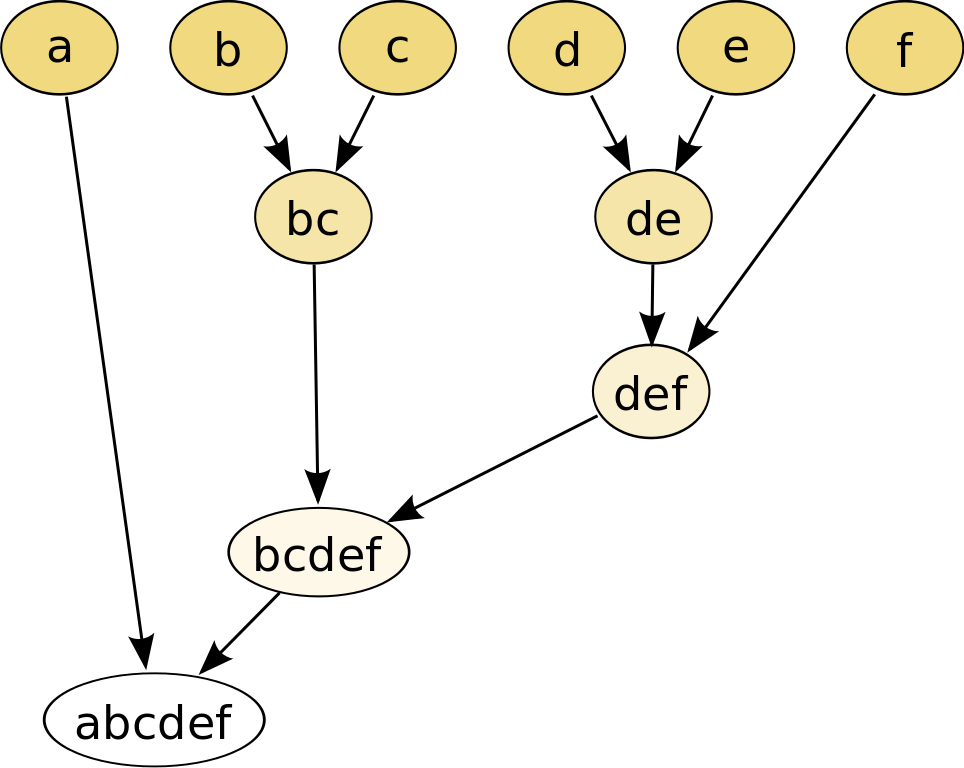
\includegraphics[height=4cm]{images/hierarchical-clustering}
\caption[Hierarchical clustering]{Hierarchical clustering}\label{fig:dendrogram}
\end{figure}



Hierarchical clustering is based on the idea that data points that are close together in feature space should be grouped together. The process starts by considering each point to be a cluster of size one. The two clusters that are closest together are then combined into a new cluster. This process continues until all points form one cluster. This produces a tree of clusters called a dendrogram (see \autoref{fig:dendrogram}). A dendrogram can be created bottom up (agglomerative clustering), as described, or top down (divisive clustering) where a single cluster is recursively split. Each level in the dendrogram is marks the distance where two clusters merged. A number of clusters can be produced by setting an appropriate merge or split threshold. Hierarchical clustering has an advantage over other methods in that the number of clusters do not have to be predetermined. The algorithm however has a complexity of $O(n^3)$ which makes it inappropriate for all but small datasets.

\begin{figure}
\centering
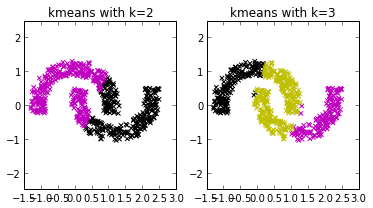
\includegraphics[height=4cm]{images/kmeans}
\caption[Hierarchical clustering]{K-means clustering \protect\footnotemark}\label{fig:kmeans}
\end{figure}

\footnotetext{Source: \url{https://pafnuty.wordpress.com/2013/08/14/non-convex-sets-with-k-means-and-hierarchical-clustering/}}


K-means clustering is computationally less expensive than hierarchical clustering. The disadvantage is that the number of clusters needs to be known upfront. An inappropriate choice can lead to bad results. The basic idea is to select K centroids and create groups by associating each input point with one of the centroids. The aim is to assign points to groups such that the average distance from a point to it's centroid is minimized. Because this optimisation is NP-hard, implementations use heuristics to compute approximate solutions \cite{Ponce2012}. K-means clustering is also limited in that it cannot deal with non convex sets (see \autoref{fig:kmeans}).

The high cost of agglomerative clustering can be overcome by first over segmenting a dataset with k-means clustering. The if the number of clusters produced k-means clustering is small enough the $O(n^3)$ cost of hierarchical clustering may be low enough to be practical.


Density-based clustering is another class of algorithms in which clusters are defined by areas of high point density. Mean-shift clustering \cite{Comaniciu2002} is an iterative approach where a kernel function is used to compute the centroid over an area of influence. For each iteration kernel is moved in the direction of the centroid until a local maxima is reached. Each point that converges to the same local maxima is assigned to a cluster. Mean shift can find arbitrary shaped clusters and the number of clusters do not have to be specified before hand. DBSCAN \cite{Ester1996} has similar properties but only requires a single pass and is thus computationally less expensive. Density based clustering algorithms pose a problem when applied to range images as the point density is non uniform. 


\begin{figure}
\centering
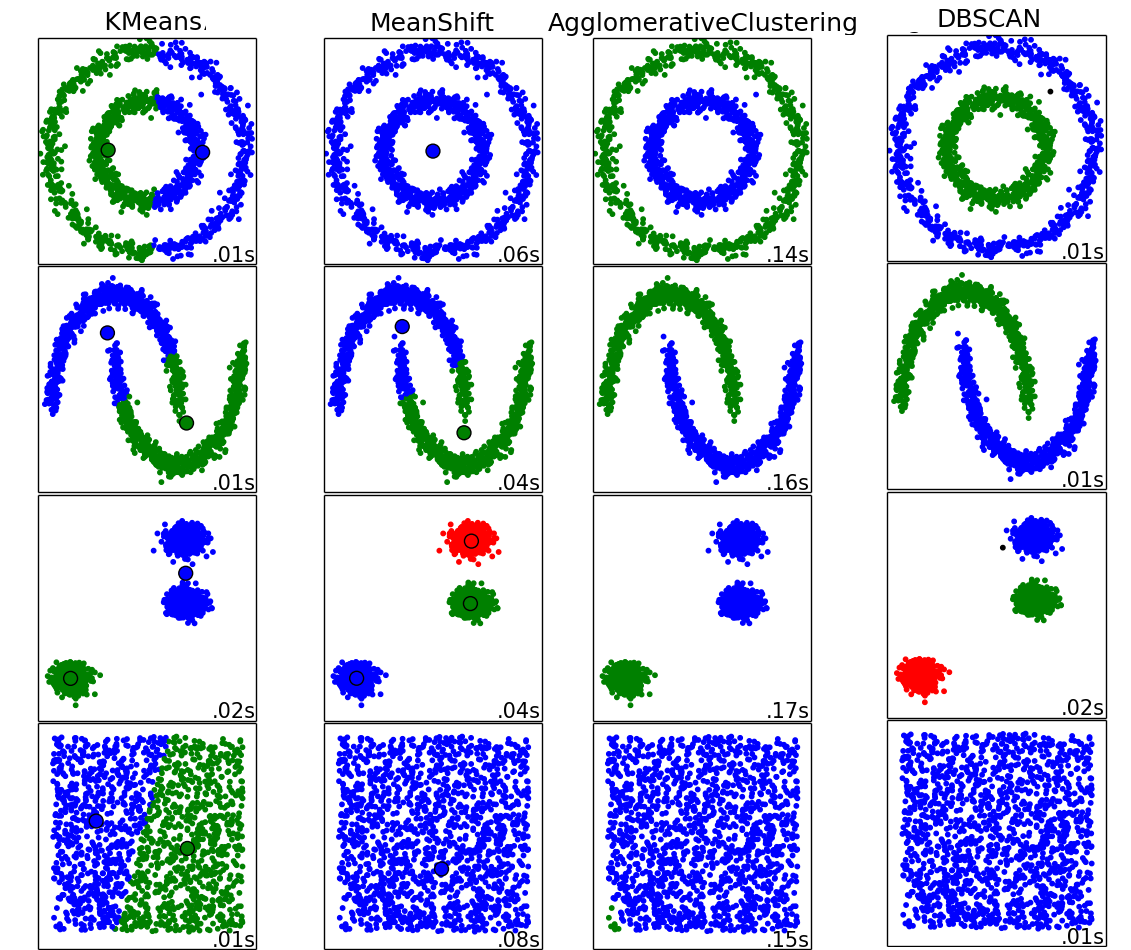
\includegraphics[height=10cm]{images/cluster-comparison}
\caption[Clustering algorithms]{Comparing different clustering algorithms on toy datasets \protect\footnotemark}\label{fig:compareclustering}
\end{figure}

\footnotetext{Adapted from: \url{http://scikit-learn.org/stable/auto_examples/cluster/plot_cluster_comparison.html}}

\subsection{Segmentation as graph partitioning}

When applying clustering algorithms to vision segmentation problems, some level of object coherence is expected. One is therefore likely to compare points that are close together. Clustering therefore naturally lends itself to being represented as a graph partitioning problem where neighbouring points are locally connected via edges that represent similarity.


\citet{Felzenszwalb2004} demonstrates this graph theoretic approach in the segmentation of 2D images. Each pixel is represented by a vertex and edge weights of neighbouring pixels indicate their dissimilarity. Each pixel is initially a cluster of one and the algorithm iterates over the edges in non decreasing order. If an edge spans two clusters and the edge weight is less than the internal difference between the clusters, the two are merged. The internal difference of a cluster is the largest edge weight inside it plus a biasing term gives small clusters higher weights.

Graph cuts are useful when a segmentation can be expressed as an energy minimisation problem. The idea is that each graph edge has a cost associated with it. Two vertices that are not part of the original graph are designated as the source and the sink (see \autoref{fig:graphcut}). Existing vertices are connected the source and the sink via weighted edges. The aim is then to separate the graph into two sub graphs containing the source and the sink by cutting the edges with the minimum cost. Segmentation tasks are typically formulated such some object is associated with the sink, and another object is associated with the source. The edges connecting to the source or sink indicates how strongly the vertex is associated with the source and sink. The weights between image vertices are set such that similar vertices are weighted heavily. The optimal cut is likely to include edges with lower weights. Because finding the minimum cost cut is the same as finding the maximum flow between the source and the sink, the optimisation can be performed in $O(VE^2)$ \cite{Edmonds1972}.


\begin{figure}
\centering
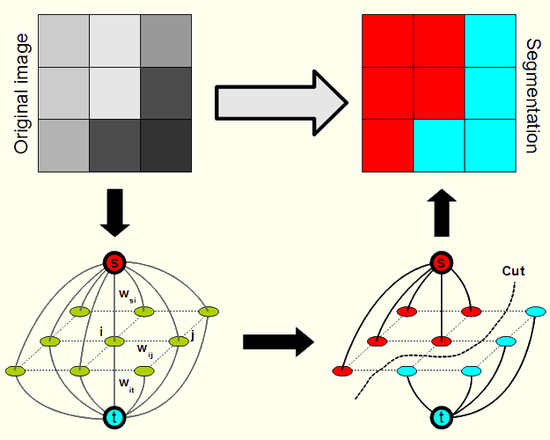
\includegraphics[height=10cm]{images/graphcut}
\caption[Graph cut]{Each pixel in the image is connected to it's neighbours, the source, and the sink. The aim of the graph cut is to remove the set of edges with the minimum weight, such that two sub graphs are created that contain the source and the sink. \protect\footnotemark}\label{fig:graphcut}
\end{figure}

\footnotetext{Source: \url{http://www.ondrej-danek.net/en/research}}


\citet{Boykov2001b} showed how graph cuts can be effectively used to perform foreground background segmentation on raster images by labelling part of the foreground and background. \citet{Boykov2001a} generalised this method to N-dimensional images and demonstrated how it can be used interactively to improve segmentation results in 2D raster images. Naive graph cuts sometimes do not perform well because the optimisation to cuts of smallest possible part of the graph in order to minimise the cut. So solve this issue \citet{Malik2000} proposed Normalised cuts in which the cost of the cut takes into account the affinity of the two graphs that would be created by a cut. That is to ensure that the two created graphs have have strong internal edge weights and weak edge weights between each other.



\subsection{Segmentation as classification}

% Grab cut

% forming image regions (sometimes use as the exclusive meaning of segmentation)
% 	decompose an image into regions that have roughly coherent color and texture.
% 	Typically, the shape of these regions isn’t particularly important, but the coherence is important
% 	regions allow us to deal with larger areas of an image without considering each element. (summary representation)
% 	super pixels can expose structure in images



% Clustering can be applied to points or groups of points

\subsection{Model driven segmentation}

Not all segmentation tasks can be performed by grouping of elements that are similar. It is often necessary to combine elements that conform to some model instead of, or in addition to clustering.

The Hough transform is a well known instance of when parametric model needs to be considered in order to segment create a segmentation that conforms to a model \cite{Ballard1981}. The Hough transform can however be prohibitively expensive to compute for all but the simplest models.

Model fitting is typically approached by trying to minimize an error function that indicates how well data conforms. Mean least squares simple way to achieve this. If we were trying to fit a plane to some data set, computing the squared error term for each point's deviation from plane. This would give us an indication of how well the plane fits the data. Given is information we could iteratively make adjustments to the plane's orientation and position in until a good fit is achieved.

This process would be significantly faster if we had a good original estimate of where the plane was. Pre-computing useful features such as corners or other key points can help register a model to good initial estimate. Clustering the data into higher level abstractions also reduces the computational workload \todo{cite that heritage paper}.

In practise data is noisy and outliers can make otherwise well behaved data not fit the model. RANSAC \cite{Fischler1981} is a fitting procedure that takes this variability into account. First one needs to determine what is the minimum number of points ($n$) one need to represent the abstraction one needs to identify. For a line $n$ would be 2, and for a plane or a sphere $n$ would be 3. Some threshold distance $t$ then needs to picked. Points further than $t$ will not be considered as fitting the model. Finally it needs to be decided how many samples is needed to confirm a model and how many outliers will be tolerated. The procedure is then to sample $n$ points at random and fit the model to them. Points are then selected at random until the model can be confirmed or rejected according to the predetermined parameters.

\todo{Tree models of canopies}
\todo{Kinect example}
\todo{Active contour model?}
\todo{Gaussian mixture model?}



\subsection{Applications}

Points that represent vegetation is undoubtedly some of the hardest classes of points to classify. Some of the most successful approaches to isolating vegetation have used scanners capable of full wave form analysis \cite{Reitberger2009, Elseberg2011}. These special scanners can detect multiple echos per emitted laser pulse. Multiple laser echos occur when more than one surface reflects the pulse. When scanning vegetation multiple echo's occur frequently because of their structure.\\

\citet{Elseberg2011} demonstrated that full wave form analysis can be used to achieve 95\% accuracy when segmenting trees from terrestrial scans on a university campus. It is unclear whether individual or merged ranges scans are used. The algorithm first projects all points to the ground plane and creates an occupancy grid. Points in in each cell are then classified as vegetation or not according to the pulse characteristics in the cell. The segments are then refined with a two pass clustering algorithm that ensures connected components have the same label. To further refine the segmentation the ratio of the two largest principle components of clusters were used distinguish trees from planar structures. A second approach to refining the clusters was adapted from \citet{Reitberger2009}. It computed a point density histogram along the vertical plane of clusters. The histogram was used with a support vector machine (SVM) to identify tree clusters. This approach produced less accurate results on the campus dataset.\\

The datasets in this research were not produced with full wave form scanners. The structure of vegetation will however produce variation in a range scan depth map. It is worth investigating whether this variation could potentially be exploited in a similar manner.\\

% multiple pulses
% principle components
% histograms of clusters

\citet{Reitberger2009} used the shape of the histogram to determine the height of a tree crowns in a clusters. Given the height of tree crown the number of stems could be estimated and an N-cut algorithm could be applied to separate trees in a cluster. This researched focused on segmenting individual trees in aerial scans of forests. In this instance a full wave form scanners was not essential to the segmentation algorithm but rather useful because it penetrates the forest canopy and allow trees below the canopy to be imaged. Terrestrial scanners do not need to penetrate canopies. The technique however, uses watershed segmentation on a projected point cloud to construct initial clusters. This approach is unlikely to be satisfactory when buildings, people and other objects are present. Other vegetation segmentation techniques are similarly inapplicable because the focus are in scenes with only vegetation \cite{Haugerud2001} or the targeted data sets are low density aerial scans \cite{Charaniya2004}.\\

% n-cuts

\citet{Barnea2012} describes an generic approach to extracting objects from color range scans that achieves 99\% accuracy on the test data. Problems with non uniform density is overcome by treating the scan as a panoramic image. Small holes in the image are interpolated from neighboring areas and a preset values are assigned to missing background data and larger regions. Mean shift clustering is used iteratively on individual image channels. The largest segment is removed and then the image is segmented again until no more segments above the threshold remain. Features derived from the range (sum of derivatives, sum of absolute derivatives, cornerness), color (HSV and Luv color space) and intensity (cornerness) are used in this process. The extracted segments are then classified as tree or non tree by a kNN classifier. The kNN classifier is trained with an example set using the same features. The segmentation is further refined using the a graph cut.\\

The color channels in the test data does not seem to contribute much discriminative power. A similar approach could thus be useful for our datasets that have no color information. Learning features means the no domain knowledge is required and the approach generalizes to other objects. Producing test data and training a classifier is however problematic in an interactive scenario. The upfront work required to produce test data may not be worthwhile if the resulting classifier only works on data similar to the training set. The kNN algorithm also poses problems as the optimal number of neighbors and the search radius needs to be determined. Features also need to be scaled correctly in order for the kNN classifier to work. The overhead of a classifier may not be necessary in an interactive environment if the user can easily select and remove unwanted segments.\\



% Canny edge detection is a simple instance where the image features are computed with a series of filters and then subsequently grouped in accordance with an edge model \cite{Canny1986}.

% Model must account for variation, hard to define

% Hough transform
% Ransacs
% Machine learning


% Features
% 	What is a good feature
% 	How to design or pick a good feature?
% 		Something that correlates with what you are trying to segment?
% 		Only evaluated as part of a learning/segmentation/clustering algorithm?
% Clusters
% Interactive segmentation
% Machine learning
% 	Deep nets
% 		Learn features via unsupervised
% 	SVG
% 	Random forests
% 	Graph optimasation

% Existing systems
% 	Range images
% 	Point clouds
% 	Aerial scans
% 	What features are used?
% 	Clustering
% 	Machine learning
% 	Level of accuracy
% 	Interactive?
% 	Assumptions?

